\documentclass[twocolumn]{IEEEtran}
\usepackage{graphicx}
\usepackage[utf8x]{inputenc}
\usepackage{times}
\usepackage{amssymb,amsfonts}
\usepackage[tbtags]{amsmath}
\usepackage{cite}
\usepackage{slashbox}
\usepackage{pict2e}
\usepackage{float}
\usepackage[all]{xy}
\usepackage{graphics,graphicx,color,colortbl}
\usepackage{times}
\usepackage{subfigure}
\usepackage{wrapfig}
\usepackage{multicol}
\usepackage{cite}
\usepackage{url}
\usepackage[tbtags]{amsmath}
\usepackage{amsmath,amssymb,amsfonts,amsbsy}
\usepackage{bm}
\usepackage{algorithm}
\usepackage{algorithmic}
\usepackage[centerlast, small]{caption}
\usepackage[colorlinks=true, citecolor=blue, linkcolor=blue, urlcolor=blue,
breaklinks=true]{hyperref}

\begin{document}
\title{Linealidad, Alinealidad y Teorema de Thevenin}
\author{José Fabio Lozano Ovalle Código: $222982$\\
	Wilson Orlando Macias Fuquen Código: $223101$\\
	David Ricardo Martínez Hernández Código: $261931$}
\maketitle
\markboth{Universidad Nacional de Colombia}{}
\floatname{algorithm}{Algoritmo}

\begin{abstract}
 Se realizaron circuitos para comprobar la linealidad de un resistor y la no linealidad de un bombillo, se diseño un circuito con 5 resistencias, al cual se le hallo el equivalente Thvenin y se comprobó dicho teorema. Se diseñaron varios circuitos para comprobar dichos fenómenos. Obteniendo las curvas características de un resistor lineal y no lineal.
\end{abstract}

\begin{keywords}
 Corriente, Linealidad, Mallas, Potencia, Thevenin, Voltaje.
\end{keywords}

\section{Objetivos}
\noindent
\begin{itemize}
 \item Obtener las curvas características de elementos lineales y no lineales.
 \item Resolver utilizando el método gráfico circuitos eléctricos con un elemento no lineal.
 \item Verificar experimentalmente  el teorema de Thevenin y aplicarlo para la resolución de circuitos eléctricos.
\end{itemize}

\section{Introducción}
\noindent
Los resistores que se trabajan en el laboratorio se asumen de comportamiento lineal a ciertos rangos de temperatura, en el caso de una bombilla la temperatura del filamento se encuentra a una temperatura de miles de kelvin, esto rompe por completo la linealidad del elemento, se espera comprobar dicho fenómeno en la práctica.\\
El equivalente Thevenin facilita el análisis de un circuito complejo, reduciendolo a una fuente en serie con una resistencia.

\section{Marco Teórico}
\noindent
Para el desarrollo de esta práctica es necesario conocer y comprender algunos conceptos básicos como linealidad y alinealidad.\\\\
\textbf{Linealidad}: Es la propiedad de un elemento que describe una relación lineal entre causa y efecto, aunque la propiedad es aplicable a muchos elementos de circuitos. La propiedad es una combinación mutua de la propiedad de homogeneidad y la propiedad de adición. \footnote{Definición tomada de \cite{sadiku}, página 120}\\
Para que se cumpla la propiedad de homogeneidad si la entrada es multiplicada por una constante, la salida también debe estar multiplicada por la misma constante. Por ejemplo para una resistencia la ley de Ohm relaciona la corriente $i$ y el voltaje $v$.
\begin{equation}
 v=iR
\label{equ1}
\end{equation}
\noindent
Si la corriente es incrementada por un factor $A$, entonces el voltaje también debe ser incrementado por el mismo factor.
\begin{equation}
 Av=AiR
\label{equ2}
\end{equation}
\noindent
Para la propiedad de adición la respuesta a la suma de varias entradas es igual a la suma de cada respuesta por separado
\begin{equation}
 v_1 = i_1R \ \ \ \ y \ \ \ \ v_2 = i_2R
\end{equation}
\noindent
al aplicar $( i_1 + i_2 )$ se obtiene
\begin{equation}
 v = ( i_1 + i_2 ) R = i_1 R + i_2 R = v_1 + v_2
\end{equation}
\noindent
De acuerdo a lo anterior la resistencia es un elemento lineal respecto a la corriente y el voltaje porque satisface las propiedades de homogeneidad y adición.\\\\
\textbf{Alineal} (\textit{del griego, prefijo a, negación y de la palabra latín linearis, que significa creado por líneas}): Dado que la linealidad cumple las propiedades de homogeneidad y adición, la alinealidad no cumple alguna o ninguna de ellas. Como la potencia, la cual tiene una relación cuadrática entre el voltaje y la corriente\footnote{Texto tomado de \cite{sadiku}, página 121}
\begin{equation}
 p = v^{2} i^{2} = \frac{v^{2}}{R} = i^{2} R
\label{equ3}
\end{equation}
\noindent
La relación entre potencia y voltaje o potencia y corriente es no lineal.\\\\
\noindent
Como esta práctica tiene una parte con una lampara incandescente y dicho elemento es no lineal, es decir no tiene una relación directa entre voltaje y corriente es necesario hacer una tabla y observar que clase de comportamiento tiene. La TABLA \ref{tab1} muestra dicho comportamiento \footnote{Ejemplo tomado de \cite{nahvi}, página 13.}
\begin{table}[H]
	\centering
\begin{tabular}[c]{|c||c|c|c|c|c|} \hline
$v$ (V) & $0.5$ & $1$ & $1.5$ & $2$ & $3$ \\ \hline
$i$ (mA) & $4$ & $6$ & $8$ & $9$ & $11$ \\ \hline \hline
$v$ (V) & $3.5$ & $4$ & $4.5$ & $5$ & $5.5$ \\ \hline
$i$ (mA) & $12$ & $13$ & $14$ & $15$ & $16$ \\ \hline \hline
$v$ (V) & $6$ & $6.5$ & $7$ & $7.5$ & $8$ \\ \hline
$i$ (mA) & $17$ & $18$ & $18$ & $19$ & $20$ \\ \hline
\end{tabular}
	\caption{Tabla de valores tomados del ejemplo}
	\label{tab1}
\end{table}
\noindent
Para el ejemplo de la TABLA \ref{tab1} y de acuerdo a la ecu. (\ref{equ1}) al despejar $R$ se obtiene como resultado $\frac{v}{i} = \frac{0.5}{4*10^{-3}} = 125 \Omega$, para el sexto valor $\frac{v}{i} = \frac{3.5}{12*10^{-3}} = 291.66 \Omega$ y para el último valor $\frac{v}{i} = \frac{8}{20*10^{-3}} = 400 \Omega$.\\\\
\textbf{Teorema Thevenin o Circuito equivalente Thevenin}:
Basado en un teorema desarrollado por M. L. Thevenin, ingeniero francés quien fue el primero en publicarlo en el año de $1883$. Para que el teorema de Thevenin pueda ser utilizado se necesita de un circuito lineal, representado como en la Fig. \ref{fig1}\footnote{Imagen tomada de \cite{sadiku}, página 131}
\begin{figure}[H]
	\centering
		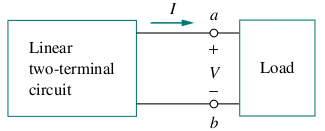
\includegraphics[scale=0.6]{th1.png}
	\caption{Representación de cajas de un circuito lineal}
	\label{fig1}
\end{figure}
\noindent
Siendo la Fig. \ref{fig2} la representación de un circuito reducido por medio del teorema Thevenin
\begin{figure}[H]
	\centering
		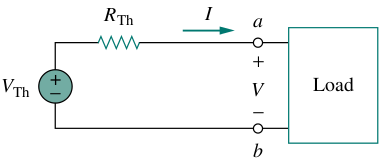
\includegraphics[scale=0.5]{th2.png}
	\caption{Representación de un circuito por el teorema Thevenin}
	\label{fig2}
\end{figure}
\noindent
El circuito a la derecha d los terminales $a - b$ es el circuito equivalente Thevenin.\\
Se establece que un circuito lineal puede ser reemplazado por una fuente de voltaje $V_{Th}$ en serie con una resistencia $R_{Th}$, para que entre los terminales $a - b$ se encuentre el voltaje esperado al analizar de una manera más sencilla un circuito. La obtención del circuito equivalente involucra varios parámetros el voltaje de circuito abierto $v_{Th}$, La corriente de corto circuito $i_{coc}$ y la resistencia de Thevenin $R_{Th}$.\\
Siendo $R_{Th}$ la resistencia equivalente del circuito vista desde las terminales $a - b$, el $v_{Th}$ el voltaje sobre la carga al ser analizada en circuito cerrado, la corriente $I$ se puede hallar por medio de la ecu. (\ref{equ4}) y el voltaje sobre la carga por medio de la ecu. (\ref{equ5})
\begin{equation}
 I_L\frac{V_{Th}}{R_{Th} + R_L}
 \label{equ4}
\end{equation}
\begin{equation}
 V_L = R_L I_L = \frac{R_L}{R_{Th} + R_L} V_{Th}
 \label{equ5}
\end{equation}

\section{Hipótesis}
\noindent
La lámpara se debe comportar como un elemento no lineal, es decir no se mantendrá constante su relación entre voltaje y corriente. \\
Para la resistencia de la lámpara incandescente se espera que a medida que el voltaje suba en sus terminales también aumente su resistencia, esta hipótesis esta basada  en el hecho del aumento de la resistencia en los metales debido al incremento en la temperatura, y como el filamento es metálico esperamos que esto se cumpla.\\
Al reemplazar un circuito por sus correspondientes equivalentes Thevenin (resistencia y voltaje), esperamos que en los extremos del  elemento, (en este caso la lámpara), se conserven iguales los voltajes y las corrientes sobre el.

\section{Materiales}
\begin{itemize}
 \item Bombillo
 \item Cables y Conectores
 \item Pinzas
 \item Protoboard
 \item Resistencias
 \item Resistor
 \item Variac
\end{itemize}


\section{Análisis y Resultados}
\subsection{Linealidad de los elementos}
\noindent
Para iniciar se utiliza el siguiente circuito sencillo usando una fuente  alterna variando su tensión a un máximo de $120 \ V_{rms}$ y tomando los datos experimentales de corriente y de esta forma obtener una gráfica de tensión contra corriente en la cual se observa la curva de un bombillo incandescente.
\begin{figure}[H]
	\centering
		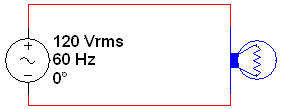
\includegraphics[scale=0.7]{b1.png}
	\caption{Montaje para hacer las medidas de voltaje-corriente en la bombilla}
	\label{fig3}
\end{figure}
\noindent
Estos fueron los valores obtenidos durante la práctica TABLA. \ref{tab1}.
\begin{table}[H]
	\centering
\begin{tabular}[c]{|c||c|c|c|c|c|c|c|c|} \hline
$v$ (V) & $0.544$ & $0.948$ & $1.501$ & $2.119$ & $2.532$ & $3.015$ & $3.45$ & $3.97$ \\ \hline
$i$ (mA) & $30$ & $47$ & $67$ & $82$ & $91$ & $98$ & $105$ & $112$ \\ \hline \hline
$v$ (V) & $4.5$ & $5.11$ & $5.51$ & $6.13$ & $6.54$ & $7.11$ & $7.58$ & $8.17$ \\ \hline
$i$ (mA) & $117$ & $123$ & $126$ & $131$ & $134$ & $138$ & $141$ & $144$ \\ \hline \hline
$v$ (V) & $8.99$ & $10.25$ & $14.57$ & $20.15$ & $25.25$ & $30.25$ & $35.0$ & $40.2$ \\ \hline
$i$ (mA) & $149$ & $156$ & $179$ & $203$ & $225$ & $245$ & $264$ & $283$ \\ \hline
$v$ (V) & $49.6$ & $60.7$ & $70.9$ & $81.4$ & $90.3$ & $100.2$ & $110.9$ & $118.8$ \\ \hline
$i$ (mA) & $315$ & $350$ & $381$ & $409$ & $432$ & $456$ & $480$ & $492$ \\ \hline
\end{tabular}
	\caption{Tabla de valores obtenidos en la práctica}
	\label{tab1}
\end{table}
\noindent
De acuerdo a la \ref{tab1}, la regresión correspondiente es una regresión exponencial, su ecuación es $y = a*{b^x}$, donde $a=160.157617$ y $b=1.001066$ y su rgafica se encuentra en la Fig. \ref{fig11}
\begin{figure}[H]
	\centering
		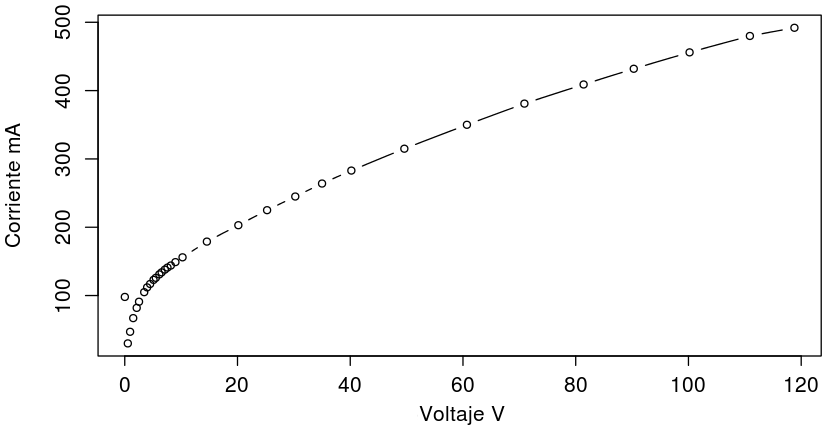
\includegraphics[scale=0.3]{reg.png}
	\caption{Función que describe el comportamiento del bombillo}
	\label{fig11}
\end{figure}
\noindent
Según los datos tomados experimentalmente consignados en la TABLA \ref{tab1} y la gráfica de la Fig \ref{fig11} obtenida a partir de estos se puede observar la curva de la bombilla, en la gráfica se puede observar que al aumentar la tensión también la corriente pero no con una relación constante, ya que la corriente aumenta la temperatura de la bombilla y así aumenta su resistencia.  De este elemento se puede decir que su comportamiento no es lineal.\\\\
Con este mismo circuito e intercambiando la bombilla por una resistencia de $100 \ \Omega$, se analiza la curva para este elemento y con la gráfica obtenida poder observar la diferencia entre los dos elementos.
\begin{figure}[H]
	\centering
		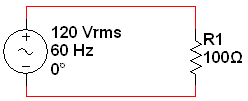
\includegraphics[scale=1]{b2.png}
	\caption{Montaje para hacer las medidas de voltaje-corriente en una resistencia}
	\label{fig4}
\end{figure}
\noindent
Estos fueron los valores obtenidos durante la práctica TABLA. \ref{tab2}.
\begin{table}[H]
	\centering
\begin{tabular}[c]{|c||c|c|c|c|c|} \hline
$v$ (V) & $0.527$ & $4.76$ & $9.74$ & $13.65$ & $19.97$ \\ \hline
$i$ (mA) & $8$ & $49$ & $100$ & $139$ & $203$ \\ \hline \hline
$v$ (V) & $30.25$ & $39.6$ & $47.0$ & $55.2$ & $66.1$ \\ \hline
$i$ (mA) & $305$ & $398$ & $474$ & $556$ & $666$ \\ \hline \hline
$v$ (V) & $77.2$ & $88.6$ & $99.9$ & $111.8$ & $118.4$ \\ \hline
$i$ (A) & $0.778$ & $0.892$ & $1.007$ & $1.127$ & $1.194$ \\ \hline
\end{tabular}
	\caption{Tabla de valores obtenidos en la práctica}
	\label{tab2}
\end{table}
\noindent
Para los datos de la TABLA \ref{tab2} representados en la gráfica, se puede ver que la resistencia de $100 \ \Omega$ tiene un comportamiento aproximadamente lineal  ya que en esta el aumento de temperatura por el paso de la corriente no es considerable y la resistencia se mantiene constante. La relación de aumento entre la tensión y la corriente es constante.
\begin{figure}[H]
	\centering
		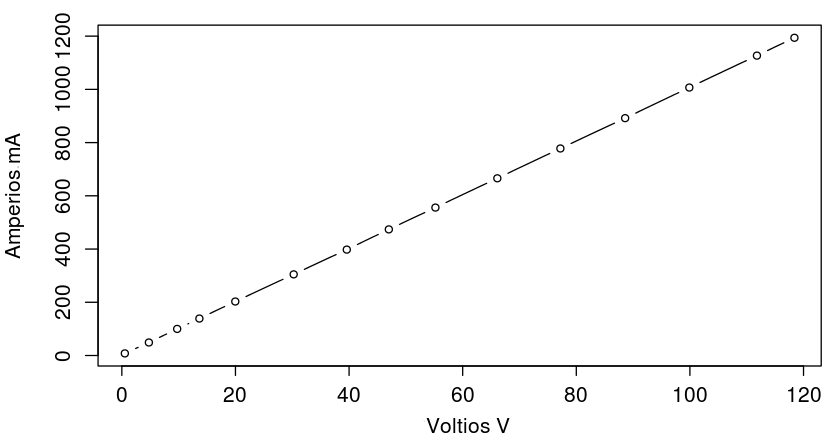
\includegraphics[scale=0.3]{res.png}
	\caption{Función que describe el comportamiento de la Resistencia descrita en la TABLA \ref{tab2}}
	\label{fig13}
\end{figure}

\subsection{Teorema Thevenin}
\noindent
En esta parte se utiliza el siguiente circuito con $5$ resistencias en serie y paralelo, identificando los puntos $A$ y $B$,  se conecta entre estos una bombilla de $60 \ w$ para la cual se analiza el sistema  con ayuda la gráfica obtenida anteriormente se puede identificar el punto de trabajo esto comparando con los datos que se obtienen experimentalmente.
\begin{figure}[H]
	\centering
		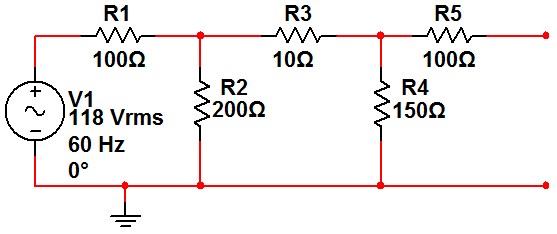
\includegraphics[scale=0.4]{m3.png}
	\caption{Montaje para Thevenin}
	\label{fig5}
\end{figure}
\noindent
Para este circuito se halla un circuito equivalente Thevenin con las ecuaciones de las mallas del circuito anterior, en el cual se conecta nuevamente la bombilla entre los puntos A y B para hacer el análisis hecho para el circuito anterior.
\begin{figure}[H]
	\centering
		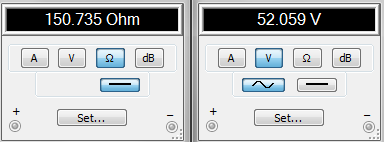
\includegraphics[scale=0.5]{r1.png}
	\caption{Resultado de la simulación del circuito Thvenin}
	\label{fig6}
\end{figure}
\noindent
Al tener la tensión ($V_{th}$) entre $A$ y $B$, y corriente del corto circuito entre los mismos puntos, se puede obtener la resistencia Thevenin ($R_{th}$) con la ley de ohm.
\begin{figure}[H]
	\centering
		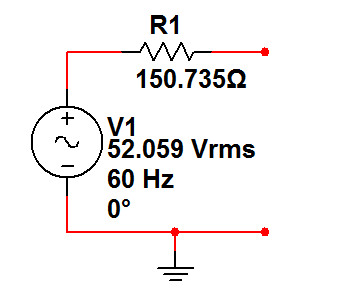
\includegraphics[scale=0.5]{th3.png}
	\caption{Resultado final del circuito Thvenin}
	\label{fig7}
\end{figure}
\begin{equation}
 120 = i_1*1.1 k - i_2 * 1 k
\end{equation}
\begin{equation}
 0 = i_2 * 2.1 k - i_1 * 1 k - i_3 * 100
\end{equation}
\begin{equation}
 0 = i_3 * 1.1 k - i_2 * 100
\end{equation}
\noindent
Los datos teóricos de los circuitos no son posibles de obtener con un software de simulación de circuitos ya que no se encuentra un elemento que se comporte similar a la bombilla, es decir con la misma curva característica entre tensión $[V]$ y corriente $[A]$.\\
\noindent
De acuerdo al análisis teórico se realizo el montaje de la Fig. \ref{fig7}, con valores muy aproximados a los valores nominales mostrados en la TABLA. \ref{tab3}
\begin{table}[H]
	\centering
\begin{tabular}[c]{|c||c|} \hline
Corriente $i_b$ $[A]$ & $0.23$ \\ \hline
Tensión $v_b$ $[V]$ & $21.5$ \\ \hline
Resistencia $R_{TH}$ $[\Omega]$ & $105.8$ \\ \hline
Tensión $v_{TH}$ $[V]$ & $52.9$ \\ \hline
\end{tabular}
	\caption{Valores obtenidos en la práctica para el Circuito Thevenin}
	\label{tab3}
\end{table}
\noindent
\begin{table}[H]
	\centering
\begin{tabular}[c]{|c||c|} \hline
Corriente $i_b$ $[A]$ & $0.23$ \\ \hline
Tensión $v_b$ $[V]$ & $20.67$ \\ \hline
Tensión $V_{fuente}$ $[V]$ & $105.8$ \\ \hline
\end{tabular}
	\caption{Valores obtenidos en la práctica para el Circuito Thevenin y el bombillo}
	\label{tab4}
\end{table}
\noindent
En los datos que se obtienen tanto del  circuito  de la Fig \ref{fig5} como de la Fig \ref{fig7} consignados en la TABLA \ref{tab1} y la TABLA \ref{tab2} se puede observar  que la tensión y corriente a través de la bombilla son aproximadamente iguales, es decir que estos circuitos son equivalentes entre sí, además se puede observar el punto de trabajo con base en la gráfica obtenida anteriormente en la Fig \ref{fig11}.
\begin{figure}[H]
	\centering
		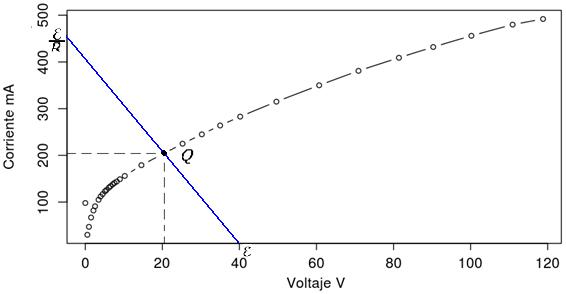
\includegraphics[scale=0.6]{final2.png}
	\caption{Punto de trabajo del bombillo en el circuito Thevenin}
	\label{fig21}
\end{figure}

\section{Preguntas}
\begin{enumerate}
 \item ¿Que  tan  lineal  es  la  resistencia  de  una  lámpara  incandescente  y  una  resistencia  de  laboratorio? ¿Se  puede  cuantificar?\\
Una resistencia se considera lineal si la razón entre la tensión aplicada en sus extremos y  la corriente que pasa a través de esta es un valor fijo, ósea si su resistencia se mantiene constante. Esta representación matemática de un fenómeno real   se puede aplicar en determinados casos, por ejemplo cuando la temperatura del resistor se mantiene constante, ya que cuando cambia la temperatura en un metal  su  resistencia se incrementa.\\
Para el caso de una lámpara incandescente su resistencia se comporta de forma no lineal ya que la temperatura del filamento se eleva a miles de grados kelvin.\\
El valor de la resistencia se puede medir en el laboratorio pero cambiara dependiendo de la temperatura del filamento.
 \item ¿Cómo se utilizan las ecuaciones de circuitos para resolver sistemas no lineales? Explique.
\begin{figure}[H]
	\centering
		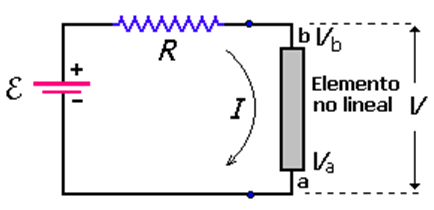
\includegraphics[scale=0.5]{l1.png}
	\caption{Circuito lineal}
	\label{fig8}
\end{figure}
Tenemos que la potencia de un elemento está dada por $P=VI$, también tenemos expresiones derivadas de la ley de Ohm, $P=V^2/R$ y $P=I^2R$. Siendo P la potencia que disipa nuestro elemento no lineal, así  tenemos:
\begin{equation}
 P = I^2 R_B
\label{ecu10}
\end{equation}
\noindent
Ya que el circuito está en serie, la corriente que circula a través de la bombilla será la misma corriente a través del resistor $R$. Por ley de Ohm tenemos que  $I = \frac{E}{R_T}$, donde $R_T$ es la suma de las dos resistencias del circuito: $R + R_B$, donde $R_B$ es la resistencia de la bombilla y E la tensión de la fuente. Por tanto:
\begin{equation}
 I = \frac{E}{(R + R_B)}
\label{equ11}
\end{equation}
\noindent
Sustituyendo (\ref{equ11}) en (\ref{ecu10}) tenemos:
\begin{equation}
\footnotesize{
 P = {\left[ {\frac{E}{{R + {R_B}}}} \right]^2}{R_B} = \left[ {\frac{{{E^2}}}{{{{\left( {R + {R_B}} \right)}^2}}}} \right]{R_B} = \frac{{{E^2}{R_B}}}{{{R^2} + 2R{R_B} + {R_B}^2}}}
\label{equ12}
\end{equation}
\noindent
Ahora, despejando el valor de $R_B$ y multiplicando ambos lados de la ecuación por $P$, y restando $E^2R_B$ tendremos finalmente la ecuación (\ref{equ13}), que nos permitirá calcular el valor de la resistencia para una tensión determinada aplicada por el circuito
\begin{equation}
 P{R^2}_B + \left( {2PR - {E^2}} \right){R_B} + P{R^2} = 0
\label{equ13}
\end{equation}
 \item ¿Qué diferencias existen entre los valores calculados por las ecuaciones y los valores experimentales en un sistema no lineal?\\
Los valores son muy similares, dado que se comportan de manera exponencial, además ese era el comportamiento esperado, porque la bombilla aumenta o reduce su resistencia, eso depende de la construcción, las propiedades del material, la composición del filamento interno.
 \item ¿Cómo se utiliza el método gráfico para solucionar sistemas no lineales?\\
Podemos también usar la ecuación que caracteriza la resistencia de un filamento de metal (tal y como lo es el filamento interno de una bombilla):
\begin{equation}
 R_b = R_o(1+a(T-T_o))
\label{equ10}
\end{equation}
\noindent
Donde:\\
$R_o$ es la resistencia en una temperatura inicial $T_o$\\
$R_b$ es la resistencia en la  temperatura final $T$\\
$a$ es el \textbf{coeficiente de temperatura de la resistividad eléctrica} (que para un filamento de tungsteno es de $4.5 x 10^{-3} \ °C^{-1}$)\\
Usando la ley de Ohm, podemos despejar la resistencia en función de la tensión  y la corriente:
\begin{equation}
 V = I{R_0}\left( {1 + a\left( {T - {T_0}} \right)} \right)
\label{equ14}
\end{equation}
\noindent
Es la ecuación (\ref{equ14}) la que usaremos para verificar  el método gráfico. La curva característica de esta ecuación es la siguiente:
\begin{figure}[H]
	\centering
		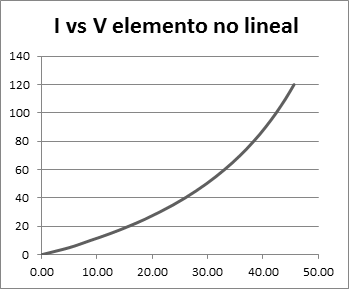
\includegraphics[scale=0.7]{g1.png}
	\caption{Curva característica ecuación \ref{equ14}}
	\label{fig9}
\end{figure}
\noindent
Usando de nuevo el circuito de la fig. \ref{fig9},  donde podemos hallar las ecuaciones propias del circuito:
\begin{equation}
 I=\frac{E}{R} - \frac{V_b}{R_b}
\label{equ15}
\end{equation}
\noindent
Para el elemento no lineal del circuito, se cumple que la corriente y el voltaje están relacionados mediante la curva característica dada en (\ref{equ10}). Podemos hallar los valores del elemento gráficamente: dibujando la recta correspondiente a la ecuación (\ref{equ15}) sobre la representación de la curva característica del elemento no lineal; el punto \textbf{$Q$} de intersección de las dos curvas indica el valor $V_0$ que satisface la igualdad y también, la corriente $I_0$ que circula por el circuito, ver Fig. \ref{fig10}. Al punto $Q$ se lo llama \textbf{punto de operación} y a la recta del elemento lineal: \textbf{recta de carga}.
\begin{figure}[H]
	\centering
		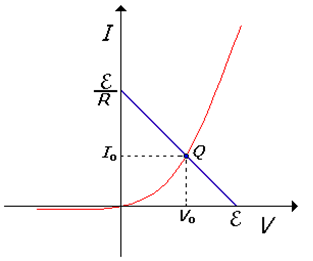
\includegraphics[scale=0.9]{f1.png}
	\caption{Función que describe el comportamiento de un elemento no lineal}
	\label{fig10}
\end{figure}
 \item ¿Existen diferencias entre los resultados del equivalente Thevenin y el sistema completo?\\
No existen muchas diferencias, el único problema fue hacer lo mas parecido posible los valores de las fuentes y de las resistencias a los valores nominales, pero son muy similares dado que los valores son muy parecidos a los nominales.
\end{enumerate}

\section{Conclusiones}
\begin{itemize}
 \item Se observa que el reóstato posee un comportamiento lineal esto se describe en las figuras de regresión lineal, mientras el bombillo presenta un comportamiento exponencial, porque la resistencia depende de la temperatura interna del bombillo, de las propiedades y los materiales con los que se encuentra construido el filamento.
 \item El equivalente Thevenin de esta práctica necesitaba valores adecuados para poder suministrar la potencia necesaria al bombillo para que encendiera, de lo contrario no se podía hacer el análisis respectivo.
 \item Las corrientes que se manejaban eran muy altas y las resistencias tenían un valor muy bajo, esto quiere decir que la potencia consumida era muy alta y tocaba tener mucho cuidado al momento de elegir las resistencias utilizadas.
 \item Los valores de voltaje y corriente medidos en la bombilla con el circuito completo, y los medidos con el equivalente Thevenin fueron muy similares. Con respecto a los valores teóricos variaron un poco debido a la potencia disipada por las resistencias y el resistor.
\end{itemize}

\bibliographystyle{ieeetran}
\begin{thebibliography}{99}
\bibitem{dorf} Dorf  \& Svoboda.
{\em "`Circuitos Eléctricos"'}.
Alfaomega, Sexta Edición, 2006.

\bibitem{sadiku} Alexander, Charles K. \&  Sadiku, Matthew N.O.
{\em "`Fundamentals of Electric Circuits"'}.
McGRAW-HILL, ISE Editions, 1999.

\bibitem{nahvi} Nahvi, Mahmood \& Edminister, Joseph A.
{\em "`Theory and Problems of Electric Circuits"'}.
McGRAW-HILL, Fourth Edition, 2003.
\end{thebibliography}
\end{document}